\documentclass{article}
\usepackage[T1]{fontenc}
\usepackage{lmodern}
\usepackage{graphicx}
\usepackage{amsmath,amssymb}
\usepackage[a4paper,margin=2cm]{geometry}
\usepackage[absolute,overlay]{textpos}
\setlength{\TPHorizModule}{1mm}
\setlength{\TPVertModule}{1mm}
\usepackage[indonesian]{babel}
\usepackage{hyperref}
\setlength{\emergencystretch}{2em}
% unit: Halaman 34

\begin{document}

% === Halaman 34 (llm) ===

\begin{itemize}
    \item Untuk membuat enkripsi menjadi lebih kompleks, gunakan kata kunci sepanjang $n$ dengan huruf-huruf berbeda. Urutan huruf di dalam kata kunci menentukan urutan pembacaan secara vertikal.
    \item Contoh: kata kunci = TOMBAK (urutan huruf sesuai alfabet: 6 5 4 2 1 3)
\end{itemize}

Plainteks: sistem dan teknologi informasi itb

\vspace{124.74mm}

Enkripsi:

\vspace{10mm}

Cipherteks: (baca secara vertikal sesuai urutan huruf di dalam kata kunci $\to 5, 4, 6, 3, 2, 1$)
\textcolor{red}{EEGRTTTOOIMKIMBSNLFIIAONSSDNIA}

% deskripsi: Ilustrasi proses enkripsi kolom dengan kata kunci TOMBAK, menunjukkan pemetaan huruf plainteks ke dalam grid berdasarkan kata kunci.
% bbox normalisasi: [0.1400, 0.4400, 0.2500, 0.8600]
\begin{textblock*}{23.10mm}(29.40mm,130.68mm)
\noindent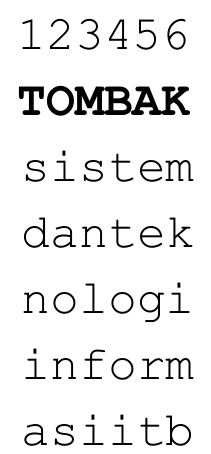
\includegraphics[width=23.10mm,height=124.74mm]{../../images/llm/page_034_img_01.png}%
\end{textblock*}

\end{document}
